% Exact visual transcription of Xi Yin, Physics 253a,
% original note pp. 30--51; combined source PDF physical pp. 41--62.
% Combined source PDF:
%   /Users/wlancer/Desktop/IAS/phy/qft/qft_253abc_book.pdf
% Source SHA-256:
%   9e5e4d241fffffa56c1c3df6dce4b83178f75787dd5d794a18c5d0c087769f21
%
% This is a literal source-layer capture. Source order, line fragments,
% punctuation, colors, arrows, braces, corrections, questions, and diagrams
% are retained. Mathematical notation is not silently normalized.
%
% Open readings are tied to:
%   work/253a-ch02/ambiguities.md
%
% Compilation requirements for reconstructed diagrams and annotations:
%   xcolor, tikz, tikz libraries arrows.meta, positioning,
%   decorations.pathmorphing.

\providecommand{\YinPageBoundary}[2]{%
  \clearpage
  \noindent\textsf{[Original Physics 253a note p.~#1; combined PDF physical p.~#2]}%
  \par\medskip
}
\providecommand{\YinLine}[1]{\noindent #1\par}
\providecommand{\YinIndent}[1]{\noindent\hspace*{2em}#1\par}
\providecommand{\YinBullet}[1]{\noindent\hspace*{1em}$\bullet$\hspace{0.7em}#1\par}
\providecommand{\YinDash}[1]{\noindent\hspace*{1em}--\hspace{0.7em}#1\par}
\providecommand{\YinBlue}[1]{{\color[rgb]{0.00,0.34,0.92}#1}}
\providecommand{\YinLightBlue}[1]{{\color[rgb]{0.47,0.67,0.82}#1}}
\providecommand{\YinPurple}[1]{{\color[rgb]{0.61,0.16,0.88}#1}}
\providecommand{\YinGray}[1]{{\color[rgb]{0.58,0.58,0.58}#1}}
\providecommand{\YinIndigo}[1]{{\color[rgb]{0.24,0.13,0.52}#1}}
\providecommand{\YinGreen}[1]{{\color[rgb]{0.00,0.52,0.22}#1}}
\providecommand{\YinRed}[1]{{\color[rgb]{0.95,0.18,0.10}#1}}
\providecommand{\YinMagenta}[1]{{\color[rgb]{0.75,0.00,0.55}#1}}
\providecommand{\YinOrange}[1]{{\color[rgb]{0.95,0.43,0.00}#1}}
\providecommand{\ket}[1]{\lvert #1\rangle}
\providecommand{\bra}[1]{\langle #1\rvert}
\providecommand{\braket}[2]{\langle #1\mid #2\rangle}

% ---------------------------------------------------------------------------
\YinPageBoundary{30}{41}

\begin{center}
  \underline{Example 2}\hspace{3em}
  \textquotedblleft an harmonic oscillator\textquotedblright
\end{center}

\[
 H=\frac{p^2}{2}+\frac{q^2}{2}+\frac{1}{4!}gq^4
 \quad\longleftrightarrow\quad
 L=\frac{1}{2}\dot q^{\,2}-\frac{q^2}{2}-\frac{1}{4!}gq^4.
\]

\YinLine{Study its Spectrum using}

\[
 \left\langle 0\middle|\widehat q(\tau)\widehat q(0)\middle|0\right\rangle
 \qquad (\tau>0)
\]

\YinBlue{%
\[
 \left\langle 0\middle|\widehat q(\tau)\widehat q(0)\middle|0\right\rangle
 =\sum_n
 \left|\left\langle n\middle|\widehat q(0)\middle|0\right\rangle\right|^2
 e^{-E_n\tau}
\]}

% The source has a single thick black curved arrow from the spectral sum to
% the path-integral line. Its exact curvature is not assigned a symbol.
\begin{center}
\begin{tikzpicture}[>=Stealth]
  \node (top) at (0,0) {};
  \node (bottom) at (0,-1.0) {};
  \draw[->,line width=1.0pt] (-0.9,0.25) .. controls (-1.7,-0.15)
    and (-1.7,-0.65) .. (-0.8,-1.0);
\end{tikzpicture}
\end{center}

\[
 =\frac{1}{Z}\int [Dq]\,e^{-\int d\tau\,L^E}\,q(\tau)q(0),
\]

\YinLine{where}
\[
 Z=\int [Dq]e^{-\int d\tau\,L^E}
\]
\[
 L^E=\frac{1}{2}(\partial_\tau q)^2+\frac{q^2}{2}+\frac{1}{4!}gq^4
\]

% AMBIGUITY P41-A1: retain ``an harmonic oscillator'', the strict tau>0
% condition, the operator hats, the plain [Dq] measure, and the visible
% black arrow as source readings. See work/253a-ch02/ambiguities.md.

% PAGE-TRANSITION: physical p. 40 closes with the free two-point function;
% physical p. 41 opens Example 2 and ends with the Euclidean Lagrangian used
% in the coupling expansion on physical p. 42.

% ---------------------------------------------------------------------------
\YinPageBoundary{31}{42}

\YinLine{Expand in powers of $g$,}

\[
\begin{aligned}
 Z={}&\int [Dq]\,e^{-\int d\tau\,\left(\frac{1}{2}(\partial_\tau q)^2+\frac{q^2}{2}\right)}
 \cdot\sum_{n=0}^{\infty}\frac{1}{n!}
 \left(-\frac{g}{4!}\int d\tau'\,q^4(\tau')\right)^n
\end{aligned}
\]

\YinLine{\YinRed{Assume} that we can exchange the order of}
\YinLine{$\int[Dq]$ with the expansion in $g$}
\YinOrange{\begin{flushright}
  [actually problematic,\\
   will revisit later]
\end{flushright}}

\[
 \frac{Z_g}{Z_0}
 =\sum_{n=0}^{\infty}\frac{1}{n!}
 \left(-\frac{g}{4!}\right)^n
 \int d\tau_1\cdots d\tau_n\cdot
 \left\langle(q(\tau_1))^4\cdots(q(\tau_n))^4\right\rangle_{\YinBlue{0}}
\]

\begin{center}
\begin{tikzpicture}[>=Stealth]
  \node at (0,0) {\YinBlue{computed using}};
  \node at (0,-0.45) {\YinBlue{\textquotedblleft free\textquotedblright Wick contractions}};
  \draw[blue,line width=0.8pt,decorate,
    decoration={brace,amplitude=4pt,mirror}] (-2.45,-0.05) -- (2.45,-0.05);
\end{tikzpicture}
\end{center}

\YinLine{$e.g.$}
\YinLine{$order\ g:$}
\[
 -\frac{g}{4!}\int d\tau\,\left\langle(q(\tau))^4\right\rangle_0
\]

% The lower row is the three source pairings at one quartic vertex. The X
% vertices are black and the contraction arcs are purple; the two plus signs
% are blue.
\begin{center}
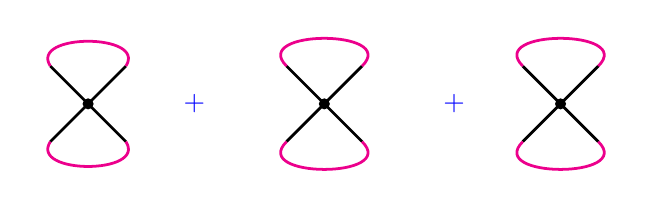
\begin{tikzpicture}[x=1cm,y=1cm]
  \foreach \x in {-3.0,0,3.0} {
    \fill (\x,0) circle (2pt);
    \draw[black,line width=1.0pt] (\x-0.48,-0.48)--(\x+0.48,0.48);
    \draw[black,line width=1.0pt] (\x-0.48,0.48)--(\x+0.48,-0.48);
  }
  \draw[magenta,line width=1.0pt] (-3.48,0.48) .. controls (-3.75,0.9)
    and (-2.25,0.9) .. (-2.52,0.48);
  \draw[magenta,line width=1.0pt] (-3.48,-0.48) .. controls (-3.75,-0.9)
    and (-2.25,-0.9) .. (-2.52,-0.48);
  \draw[blue] (-1.65,0) node {+};
  \draw[magenta,line width=1.0pt] (-0.48,0.48) .. controls (-0.95,0.95)
    and (0.95,0.95) .. (0.48,0.48);
  \draw[magenta,line width=1.0pt] (-0.48,-0.48) .. controls (-0.95,-0.95)
    and (0.95,-0.95) .. (0.48,-0.48);
  \draw[blue] (1.65,0) node {+};
  \draw[magenta,line width=1.0pt] (2.52,0.48) .. controls (2.05,0.95)
    and (3.95,0.95) .. (3.48,0.48);
  \draw[magenta,line width=1.0pt] (2.52,-0.48) .. controls (2.05,-0.95)
    and (3.95,-0.95) .. (3.48,-0.48);
\end{tikzpicture}
\end{center}

% AMBIGUITY P42-A1: retain the red Assume, the orange bracketed warning,
% the blue free-Wick annotation, the centered multiplication dots, and all
% three distinct quartic pairings. See work/253a-ch02/ambiguities.md.

% PAGE-TRANSITION: physical p. 42 ends with the order-g Wick pairings;
% physical p. 43 evaluates that term, begins the g^2 term, and leaves the
% graph-combinatorics sentence open at the lower edge.

% ---------------------------------------------------------------------------
\YinPageBoundary{32}{43}

\[
 =-\frac{g}{8}\int d\tau\,\bigl(G_0(\tau,\tau)\bigr)^2
\]
\begin{center}
\begin{tikzpicture}[>=Stealth]
  \draw[blue,->,line width=0.8pt] (0,-0.6)--(0,0.1);
  \draw[blue,line width=0.8pt,decorate,
    decoration={brace,amplitude=3pt,mirror}] (0.6,-0.05)--(2.6,-0.05);
  \node[blue] at (1.6,-0.55) {\textquotedblleft const\textquotedblright};
  \node[blue,align=left] at (1.55,-1.15)
    {diverges as $\tau\mathbin{->}\pm\infty$,\\[-1pt] will interpret later.};
\end{tikzpicture}
\end{center}

\YinLine{At order $g^2$.}
\[
 \frac{1}{2}\left(-\frac{g}{4!}\right)^2
 \int d\tau_1,d\tau_2\,
 \left\langle\bigl(\phi(\tau_1)\bigr)^4
 \bigl(\phi(\tau_2)\bigr)^4\right\rangle_0
\]

\YinLine{Two types of Wick contractions:}

\begin{center}
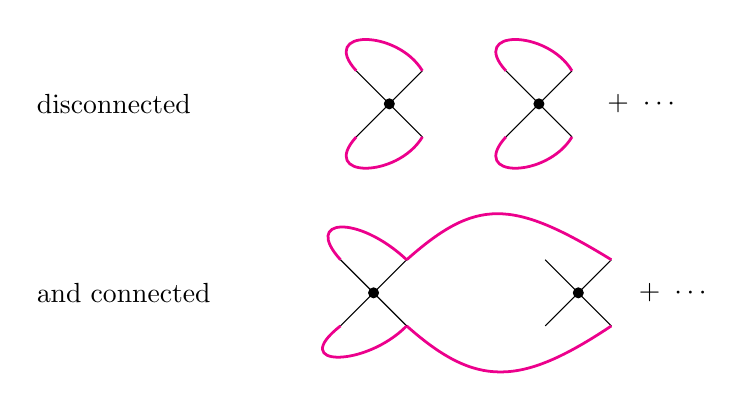
\begin{tikzpicture}[x=1cm,y=1cm]
  \node[anchor=west] at (-6.0,1.6) {disconnected};
  \foreach \x in {-1.4,0.5} {
    \fill (\x,1.6) circle (2pt);
    \draw[black] (\x-0.42,1.18)--(\x+0.42,2.02);
    \draw[black] (\x-0.42,2.02)--(\x+0.42,1.18);
    \draw[magenta,line width=1.0pt] (\x-0.42,2.02) .. controls
      (\x-0.9,2.55) and (\x+0.1,2.55) .. (\x+0.42,2.02);
    \draw[magenta,line width=1.0pt] (\x-0.42,1.18) .. controls
      (\x-0.9,0.65) and (\x+0.1,0.65) .. (\x+0.42,1.18);
  }
  \node at (1.8,1.6) {$+\ \cdots$};
  \node[anchor=west] at (-6.0,-0.8) {and connected};
  \foreach \x in {-1.6,1.0} {
    \fill (\x,-0.8) circle (2pt);
    \draw[black] (\x-0.42,-1.22)--(\x+0.42,-0.38);
    \draw[black] (\x-0.42,-0.38)--(\x+0.42,-1.22);
  }
  \draw[magenta,line width=1.0pt] (-2.02,-0.38) .. controls (-2.5,0.15)
    and (-1.8,0.2) .. (-1.18,-0.38);
  \draw[magenta,line width=1.0pt] (-2.02,-1.22) .. controls (-2.7,-1.75)
    and (-1.7,-1.75) .. (-1.18,-1.22);
  \draw[magenta,line width=1.0pt] (-1.18,-0.38) .. controls (-0.3,0.4)
    and (0.15,0.4) .. (1.42,-0.38);
  \draw[magenta,line width=1.0pt] (-1.18,-1.22) .. controls (-0.3,-2.0)
    and (0.25,-2.0) .. (1.42,-1.22);
  \node at (2.2,-0.8) {$+\ \cdots$};
\end{tikzpicture}
\end{center}

\YinLine{More generally, at order $g^n$,}
\YinLine{each set of Wick contractions can be}
\YinLine{represented by a graph that consists of}

% AMBIGUITY P43-A1: the blue quotation marks around ``const'', the brace
% endpoints, and the exact third connected pairing are visual readings only.
% See work/253a-ch02/ambiguities.md.
% AMBIGUITY P43-A2: the field glyph in the g^2 expectation is retained as
% phi/varphi according to the lane reading; no canonical replacement is made.
% See work/253a-ch02/ambiguities.md.

% PAGE-TRANSITION: physical p. 43 continues on physical p. 44 with K
% connected components and the multiplicities m_l.

% ---------------------------------------------------------------------------
\YinPageBoundary{33}{44}

\YinLine{K connected components, among them}
\YinLine{there are $m_\ell$ connected graphs that contain}
\YinLine{$\ell$ vertices each, $\ell=1,2,3,\ldots$}

\[
 \sum_{\ell\ge 1}m_\ell=K,\qquad
 \sum_{\ell\ge 1}m_\ell\cdot\ell=n.
\]
\begin{center}
\begin{tikzpicture}[>=Stealth]
  \draw[blue,->,line width=0.8pt] (0,0.3) .. controls (0.7,0.9)
    and (2.2,0.9) .. (3.0,0.3);
\end{tikzpicture}
\end{center}

\YinLine{For a given such partition of $n$,}
\YinLine{specified by $m_\ell$'s, the number of ways}
\YinLine{of grouping the $n$ vertices in this pattern}
\YinLine{is}
\[
 \frac{n!}{\prod_{\ell\ge 1}(\ell!)^{m_\ell}\cdot m_\ell!}
\]

\YinLine{Total contribution is}
\[
 \frac{1}{n!}
 \frac{n!}{\prod_{\ell\ge 1}(\ell!)^{m_\ell}\cdot m_\ell!}
 \prod_{\ell\ge 1}\left(G^{(\ell)}\right)^{m_\ell}
\]
\[
 =\prod_{\ell\ge 1}\frac{1}{m_\ell!}
 \left(\frac{1}{\ell!}G^{(\ell)}\right)^{m_\ell}
\]
\begin{center}
\begin{tikzpicture}[>=Stealth]
  \draw[blue,->,line width=0.8pt] (0,0)--(0.45,0.55);
\end{tikzpicture}
\end{center}

% AMBIGUITY P44-A1: retain the centered denominator dots and the scope of
% the product exactly as written. See work/253a-ch02/ambiguities.md.
% PAGE-TRANSITION: physical p. 44 points from G^{(ell)} to its definition on
% physical p. 45, where the partition sum is exponentiated.

% ---------------------------------------------------------------------------
\YinPageBoundary{34}{45}

% An isolated blue hooked stroke appears above the first annotation. It has no
% attached word or recoverable arrowhead.
\begin{center}
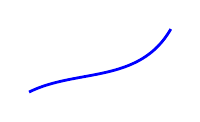
\begin{tikzpicture}
  \draw[blue,line width=1.0pt] (0,0) .. controls (0.6,0.3)
    and (1.4,0.1) .. (1.8,0.8);
\end{tikzpicture}
\end{center}

\begin{center}
\YinBlue{$G^{(\ell)}$ is the contribution from}\\[-2pt]
\YinBlue{connected Wick contraction of}\\[-2pt]
\YinBlue{$\ell$ vertices}
\end{center}

\[
 \frac{Z_g}{Z_0}
 =\sum_{\{m_\ell\}}\prod_{\ell\ge 1}
 \frac{1}{m_\ell!}\left(\frac{1}{\ell!}G^{(\ell)}\right)^{m_\ell}
\]
\[
 =\prod_{\ell\ge 1}\exp\left(\frac{1}{\ell!}G^{(\ell)}\right)
\]
\[
 =\exp\left(\sum_{\ell\ge 1}\frac{1}{\ell!}G^{(\ell)}\right)
\]

\begin{center}
\begin{tikzpicture}[>=Stealth]
  \draw[blue,line width=0.8pt,decorate,
    decoration={brace,amplitude=4pt,mirror}] (-2.0,0)--(2.0,0);
  \node[blue,align=center] at (0,-0.7)
    {contribution from all\\ connected graphs};
\end{tikzpicture}
\end{center}

\begin{center}
\YinBlue{$e.g.$}
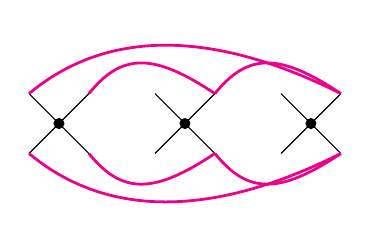
\begin{tikzpicture}[x=1cm,y=1cm]
  \foreach \x in {-1.6,0,1.6} {
    \fill (\x,0) circle (2pt);
    \draw[black] (\x-0.38,-0.38)--(\x+0.38,0.38);
    \draw[black] (\x-0.38,0.38)--(\x+0.38,-0.38);
  }
  \draw[magenta,line width=1.0pt] (-1.98,0.38) .. controls (-1.0,1.2)
    and (0.35,1.2) .. (1.98,0.38);
  \draw[magenta,line width=1.0pt] (-1.98,-0.38) .. controls (-1.0,-1.2)
    and (0.35,-1.2) .. (1.98,-0.38);
  \draw[magenta,line width=1.0pt] (-1.22,0.38) .. controls (-0.8,0.9)
    and (-0.4,0.9) .. (0.38,0.38);
  \draw[magenta,line width=1.0pt] (-1.22,-0.38) .. controls (-0.8,-0.9)
    and (-0.4,-0.9) .. (0.38,-0.38);
  \draw[magenta,line width=1.0pt] (0.38,0.38) .. controls (0.8,0.9)
    and (1.2,0.9) .. (1.98,0.38);
  \draw[magenta,line width=1.0pt] (0.38,-0.38) .. controls (0.8,-0.9)
    and (1.2,-0.9) .. (1.98,-0.38);
\end{tikzpicture}
\end{center}

\YinBlue{\[
\begin{aligned}
={}&\frac{1}{3!}\left(-\frac{g}{4!}\right)^3
 \int d\tau_1\,d\tau_2\,d\tau_3\,
 \left(G_0(\tau_1,\tau_2)\right)^2\\[-1pt]
&\cdot\left(G_0(\tau_2,\tau_3)\right)^2
 \left(G_0(\tau_3,\tau_1)\right)^2.
\end{aligned}
\]}

\YinBlue{\YinLine{Still diverges like $\int d\tau\cdot(\mathrm{Const})$.}}

% AMBIGUITY P45-A1: the isolated upper blue stroke and the case of
% ``Const'' are retained as open visual readings. See
% work/253a-ch02/ambiguities.md.

% PAGE-TRANSITION: physical p. 45 ends the connected-graph exponentiation
% example and begins a new heading, ``Interpretation of'', on physical p. 46.

% ---------------------------------------------------------------------------
\YinPageBoundary{35}{46}

\begin{center}
  Interpretation of
\end{center}

\[
\begin{aligned}
 Z&=\int [Dq]e^{-\int d\tau\,L^E}\\
  &=\langle q_f\,|\,e^{-HT}\,|\,q_i\rangle
\end{aligned}
\]

\begin{center}
\begin{tikzpicture}[>=Stealth]
  \draw[blue,->,line width=0.8pt] (-2.0,0)--(-1.3,0.35);
  \draw[blue,->,line width=0.8pt] (2.0,0)--(1.3,0.35);
  \node[blue,align=left] at (0,-0.15)
    {boundary\\ condition at initial and final\\
     imaginary time $\tau=0,T$,\\
     unspecified as we take $T\to\infty$};
\end{tikzpicture}
\end{center}

\[
 \log Z=-E_0\cdot T+O(1)
\]
\begin{center}
\begin{tikzpicture}[>=Stealth]
  \draw[blue,decorate,decoration={snake,amplitude=0.3mm,segment length=1.8mm}]
    (-0.3,0)--(0.5,0);
  \draw[blue,->] (0.1,-0.7)--(0.1,-0.05);
  \node[blue] at (0.1,-1.0) {ground state energy};
\end{tikzpicture}
\end{center}

\YinLine{Indeed, we have seen in perturbation}
\YinLine{theory.}
\[
 \log\frac{Z_g}{Z_0}=\sum_{\ell=1}^{\infty}\frac{1}{\ell!}G^{(\ell)}
\]
\begin{center}
\begin{tikzpicture}[>=Stealth]
  \draw[blue,decorate,decoration={snake,amplitude=0.3mm,segment length=1.8mm}]
    (-0.35,0)--(0.75,0);
  \draw[blue,->] (0.2,-0.65)--(0.2,-0.05);
  \node[blue,align=center] at (0.2,-1.05)
    {sum of all Wick contractions\\ of $\ell$ vertices via \underline{connected} graphs};
\end{tikzpicture}
\end{center}

\YinLine{$*$ One often absorbs the combinatorial}

% AMBIGUITY P46-A1: the endpoint arrows and the notation L^E are preserved
% without choosing a canonical boundary-condition convention. See
% work/253a-ch02/ambiguities.md.
% PAGE-TRANSITION: the starred sentence continues on physical p. 47 with
% ``factor 1/ell! into the "symmetry factor" of the graph itself.''

% ---------------------------------------------------------------------------
\YinPageBoundary{36}{47}

\YinLine{factor $\frac{1}{\ell!}$ into the \textquotedblleft symmetry factor\textquotedblright}
\YinLine{of the graph itself.}

\YinLine{$*$ each $G^{(\ell)}$ is of the form}
\[
 \int d\tau\,(\mathrm{const})\propto T.
\]

\YinLine{Thus}
\[
 E_0=-\lim_{T\to\infty}\frac{1}{T}\log Z
\]
\YinLine{is well-defined.}

\YinLine{As already seen, at order $g$, $\ell=1$.}

\begin{center}
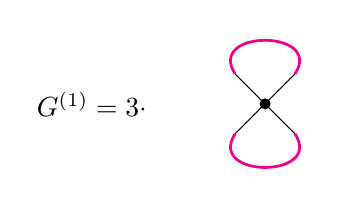
\begin{tikzpicture}[baseline]
  \node at (-1.2,0) {$G^{(1)}=3\cdot$};
  \fill (1.0,0) circle (2pt);
  \draw[black] (0.62,-0.38)--(1.38,0.38);
  \draw[black] (0.62,0.38)--(1.38,-0.38);
  \draw[magenta,line width=1.0pt] (0.62,0.38) .. controls (0.25,0.95)
    and (1.75,0.95) .. (1.38,0.38);
  \draw[magenta,line width=1.0pt] (0.62,-0.38) .. controls (0.25,-0.95)
    and (1.75,-0.95) .. (1.38,-0.38);
\end{tikzpicture}
\end{center}

\[
 =-\frac{g}{8}\cdot\int d\tau\,\bigl(G_0(\tau,\tau)\bigr)^2
\]

\begin{center}
\YinBlue{Recall}\qquad
\YinBlue{$G(\tau_1,\tau_2)=\frac{1}{2\omega}e^{-\omega|\tau_{12}|}$}
\\[4pt]
\YinBlue{$G_0(\tau,\tau)=\frac{1}{2\omega}$}
\end{center}

\[
 \Rightarrow\Delta E_0=\frac{g}{8}\cdot
 \left(\frac{1}{2\omega}\right)^2+O(g^2)
\]
\begin{center}
\begin{tikzpicture}[>=Stealth]
  \draw[blue,->] (0,0.45)--(0,0.05);
  \node[blue] at (1.3,0.4) {correction to ground state energy};
  \node[gray] at (3.2,1.0) {(have set $\omega=1$)};
\end{tikzpicture}
\end{center}

% AMBIGUITY P47-A1: the first blue propagator reminder is G rather than G_0
% in the source capture; the case of const and the exact loop strokes remain
% open. See work/253a-ch02/ambiguities.md.
% PAGE-TRANSITION: physical p. 47 ends with the path-integral energy shift;
% physical p. 48 begins ``Comparison to Hamiltonian perturbation theory:''.

% ---------------------------------------------------------------------------
\YinPageBoundary{37}{48}

\begin{center}
  Comparison to Hamiltonian perturbation theory:
\end{center}

% A small isolated black dot sits immediately before the Hamiltonian line.
\YinLine{$\cdot\quad H=\frac{\widehat p^{\,2}}{2}+\frac{\widehat q^{\,2}}{2}
 +\frac{1}{4!}g\widehat q^{\,4}$}

\begin{center}
\begin{tikzpicture}[>=Stealth]
  \draw[blue,line width=0.8pt,decorate,
    decoration={brace,amplitude=4pt,mirror}] (-2.8,0)--(-0.2,0);
  \node[blue] at (-1.5,-0.45) {$H_0$};
  \draw[blue,line width=0.8pt,decorate,
    decoration={brace,amplitude=4pt,mirror}] (0.35,0)--(2.7,0);
  \node[blue] at (1.5,-0.45) {$H_1$};
\end{tikzpicture}
\end{center}

\YinLine{Let $|\psi_0\rangle$ be ground state of $H_0$,}
\YinLine{to leading order in $g$,}
\[
\begin{aligned}
 \Delta E_0&\approx\langle\psi_0|H_1|\psi_0\rangle\\
 &=\frac{1}{4!}g\left\langle\widehat q^{\,4}\right\rangle_0
 =\frac{g}{32}.
\end{aligned}
\]
\begin{center}
\begin{tikzpicture}
  \draw[blue,line width=0.8pt,decorate,
    decoration={brace,amplitude=3pt,mirror}] (-1.6,0)--(0.1,0);
  \node[blue] at (-0.75,-0.45) {$=\frac{3}{4}$};
  \node[blue] at (1.4,0.1) {$\checkmark$};
\end{tikzpicture}
\end{center}

% AMBIGUITY P48-A1: retain the isolated black dot and the three short blue
% brace-to-label strokes as source marks, not algebraic symbols. See
% work/253a-ch02/ambiguities.md.
% PAGE-TRANSITION: physical p. 48 closes the first-order comparison at g/32;
% physical p. 49 turns to the positive-time two-point function.

% ---------------------------------------------------------------------------
\YinPageBoundary{38}{49}

\YinLine{Next we turn to}\hfill\YinLine{$(\tau>0)$}

\[
 \left\langle0\middle|\widehat q(\tau)\widehat q(0)\middle|0\right\rangle
\]
\[
 =\frac{1}{Z}\int[Dq]e^{-\int d\tau\,L^E}\cdot q(\tau)q(0).
\]

\begin{center}
\begin{tikzpicture}[>=Stealth]
  \draw[magenta,->,line width=0.9pt] (0,-1.0) .. controls (0.2,-0.4)
    and (0.9,-0.2) .. (1.1,0.25);
  \node[magenta] at (0,-1.35) {expand in $g$.};
\end{tikzpicture}
\end{center}

\[
 =\frac{1}{Z}\left\langle q(\tau)q(0)
 \sum_{n=0}^{\infty}\frac{1}{n!}
 \left(-\frac{g}{4!}\int d\tau'\,q^4(\tau')\right)^n
 \right\rangle_{\YinBlue{0}}.
\]

\begin{center}
\begin{tikzpicture}[>=Stealth]
  \draw[blue,->,line width=0.8pt] (-0.8,-0.8)--(-0.2,0.0);
  \node[blue,align=left] at (0,-1.45)
    {Computed by summing up all possible\\
     Wick contractions, consisting of terms\\ like};
\end{tikzpicture}
\end{center}

\[
 q(\tau)q(0)\left(-\frac{g}{4!}\int d\tau'\,q^4(\tau')\right)
 \left(\text{graphical Wick-contraction pattern}\right)\cdots
\]

% The purple overbrackets group the external fields, the interaction, and
% successive contraction choices. The grouped symbols are retained even
% though the individual pairings are not separately labeled in the source.
\begin{center}
\begin{tikzpicture}[x=1cm,y=1cm,>=Stealth]
  \fill[red] (-3.5,0) circle (2.5pt);
  \fill[red] (0.0,0) circle (2.5pt);
  \draw[black,line width=1.0pt] (-3.5,0)--(0,0);
  \fill ( -1.75,0) circle (2pt);
  \draw[magenta,line width=1.0pt] (-1.75,0) .. controls (-2.3,0.9)
    and (-1.2,0.9) .. (-1.75,0);
  \node[red] at (-3.5,-0.45) {$x(\tau)$};
  \node[red] at (0,-0.45) {$x(0)$};
  \draw[blue,line width=0.8pt,decorate,
    decoration={brace,amplitude=4pt,mirror}] (1.3,0.5)--(4.0,0.5);
  \node[blue,align=left] at (2.7,-0.7)
    {other disconnected\\ component of\\ the graph};
\end{tikzpicture}
\end{center}

\YinLine{The sum factorizes as}
\begin{center}
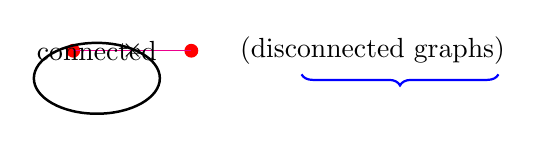
\begin{tikzpicture}[x=1cm,y=1cm]
  \fill[red] (-3.3,0) circle (2.5pt);
  \fill[red] (-1.8,0) circle (2.5pt);
  \draw[magenta] (-3.3,0)--(-1.8,0);
  \draw[black,line width=0.9pt] (-3.0,-0.35) ellipse (0.8 and 0.45);
  \node at (-3.0,0) {connected};
  \node at (-2.55,0) {$\times$};
  \node at (0.5,0) {(disconnected graphs)};
  \draw[blue,line width=0.8pt,decorate,
    decoration={brace,amplitude=4pt,mirror}] (-0.4,-0.3)--(2.1,-0.3);
\end{tikzpicture}
\end{center}

% AMBIGUITY P49-A1: the red endpoint labels in the connected example are
% captured as x(tau), x(0), although the surrounding equations use q. See
% work/253a-ch02/ambiguities.md.
% PAGE-TRANSITION: physical p. 49 leaves the connected/disconnected
% factorization open; physical p. 50 begins with Z cancelling 1/Z.

% ---------------------------------------------------------------------------
\YinPageBoundary{39}{50}

\begin{center}
\YinBlue{\textquotedblleft Z\textquotedblright}\\[-2pt]
\YinBlue{Cancels against $\frac{1}{Z}$.}
\end{center}
\YinLine{leaving the result}
\[
 \left\langle0\middle|\widehat q(\tau)\widehat q(0)\middle|0\right\rangle
\]

% The source displays the connected diagram series rather than symbolic
% names. The endpoint dots are red and the graph strokes are black.
\begin{center}
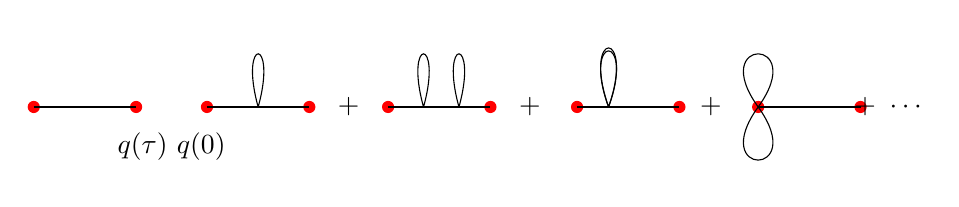
\begin{tikzpicture}[x=1cm,y=1cm]
  \foreach \x in {-5.2,-3.0,-0.7,1.7,4.0} {
    \fill[red] (\x-0.65,0) circle (2.2pt);
    \fill[red] (\x+0.65,0) circle (2.2pt);
    \draw[black] (\x-0.65,0)--(\x+0.65,0);
  }
  \draw[black] (-3.0,0) .. controls (-3.25,0.9) and (-2.75,0.9) .. (-3.0,0);
  \draw[black] (-0.9,0) .. controls (-1.15,0.9) and (-0.65,0.9) .. (-0.9,0);
  \draw[black] (-0.45,0) .. controls (-0.7,0.9) and (-0.2,0.9) .. (-0.45,0);
  \draw[black] (1.45,0) .. controls (1.1,0.95) and (1.8,0.95) .. (1.45,0);
  \draw[black] (1.45,0) .. controls (1.1,1.0) and (1.8,1.0) .. (1.45,0);
  \draw[black] (3.35,0) .. controls (2.7,-0.9) and (4.0,-0.9) .. (3.35,0);
  \draw[black] (3.35,0) .. controls (2.7,0.9) and (4.0,0.9) .. (3.35,0);
  \node at (-4.1,-0.5) {$q(\tau)\ q(0)$};
  \node at (-1.85,0) {$+$};
  \node at (0.45,0) {$+$};
  \node at (2.75,0) {$+$};
  \node at (5.0,0) {$+\ \cdots$};
\end{tikzpicture}
\end{center}

\YinGray{\YinLine{Note: Same path integral expression computes}}
\YinGray{\[
 \left\langle0\middle|\widehat q(0)\widehat q(\tau)\middle|0\right\rangle
 \qquad\text{for $\tau<0$.}
\]}
\YinGray{\YinLine{We can write the Euclidean Green function}}
\YinGray{\[
 \left\langle q(\tau)q(0)\right\rangle=
 \begin{cases}
  \left\langle0\middle|\widehat q(\tau)\widehat q(0)\middle|0\right\rangle,
    &\tau\ge0,\\[4pt]
  \left\langle0\middle|\widehat q(0)\widehat q(\tau)\middle|0\right\rangle,
    &\tau<0.
 \end{cases}
\]}

\begin{center}
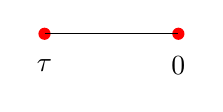
\begin{tikzpicture}
  \fill[red] (0,0) circle (2.2pt); \fill[red] (1.7,0) circle (2.2pt);
  \draw (0,0)--(1.7,0);
  \node at (0,-0.4) {$\tau$}; \node at (1.7,-0.4) {$0$};
\end{tikzpicture}
\end{center}
\[
 G_0(\tau)=\frac{1}{2}e^{-|\tau|}
\]
\YinBlue{\[
 =\int\frac{dk}{2\pi}\,\widetilde G_0(k)e^{ik\tau},
 \qquad \widetilde G_0(k)=\frac{1}{k^2+1}
\]}

% AMBIGUITY P50-A1: preserve the source distinction tau>0 on p. 49 and
% tau>=0 in the first branch here, and preserve the diagrammatic series.
% See work/253a-ch02/ambiguities.md.
% PAGE-TRANSITION: physical p. 50 ends with G_0(tau) and its Fourier form;
% physical p. 51 begins the one-loop tadpole evaluation.

% ---------------------------------------------------------------------------
\YinPageBoundary{40}{51}

\begin{center}
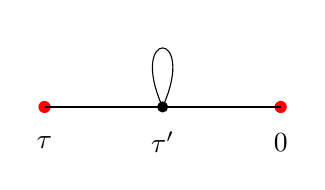
\begin{tikzpicture}
  \fill[red] (0,0) circle (2.2pt); \fill[red] (3.0,0) circle (2.2pt);
  \draw (0,0)--(3.0,0); \fill (1.5,0) circle (2pt);
  \draw (1.5,0) .. controls (1.05,1.0) and (1.95,1.0) .. (1.5,0);
  \node at (0,-0.45) {$\tau$}; \node at (1.5,-0.45) {$\tau'$};
  \node at (3.0,-0.45) {$0$};
\end{tikzpicture}
\end{center}
\[
 =-\frac{g}{2}\int d\tau'\,G_0(\tau-\tau')G_0(\tau')G_0(0)
\]

\YinLine{convenient to evaluation using Fourier transf.}
\[
\begin{aligned}
={}&-\frac{g}{2}\int d\tau'\int\frac{dk}{2\pi}\int\frac{dk'}{2\pi}
 \widetilde G_0(k)\widetilde G_0(k')
 e^{ik(\tau-\tau')+ik'\tau'}\\[-1pt]
&\cdot\int\frac{dk''}{2\pi}\cdot\widetilde G_0(k'')
\end{aligned}
\]
\[
 =-\frac{g}{2}\cdot\frac{1}{2}\int\frac{dk}{2\pi}\cdot
 \frac{e^{ik\tau}}{(k^2+1)^2}
\]

\begin{center}
\begin{tikzpicture}[>=Stealth]
  \fill (0,0) circle (2pt); \fill (2.6,0) circle (2pt);
  \draw (0,0)--(2.6,0); \fill (1.3,0) circle (2pt);
  \draw (1.3,0) .. controls (0.85,0.9) and (1.75,0.9) .. (1.3,0);
  \draw[blue,->] (0.85,-0.28)--(0.35,-0.28);
  \draw[blue,->] (2.15,-0.28)--(1.65,-0.28);
  \draw[blue,->] (1.0,0.75)--(0.82,0.35);
  \node[blue] at (0.55,-0.65) {$k$};
  \node[blue] at (2.05,-0.65) {$k'=k$};
  \node[blue] at (1.0,1.05) {$k''$};
\end{tikzpicture}
\end{center}

\YinLine{At order $g^2$, we have}
\begin{center}
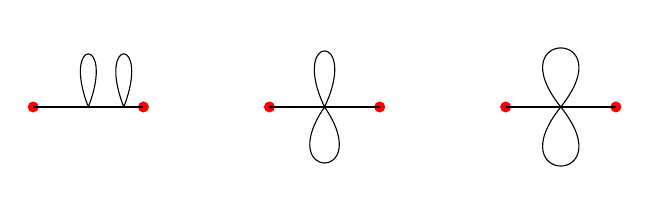
\begin{tikzpicture}[x=1cm,y=1cm]
  \foreach \x in {-3.0,0,3.0} {
    \fill[red] (\x-0.7,0) circle (2pt); \fill[red] (\x+0.7,0) circle (2pt);
    \draw (\x-0.7,0)--(\x+0.7,0);
  }
  \draw (-3.0,0) .. controls (-3.35,0.9) and (-2.65,0.9) .. (-3.0,0);
  \draw (-2.55,0) .. controls (-2.9,0.9) and (-2.2,0.9) .. (-2.55,0);
  \draw (0,0) .. controls (-0.45,0.95) and (0.45,0.95) .. (0,0);
  \draw (0,0) .. controls (-0.65,-0.95) and (0.65,-0.95) .. (0,0);
  \draw (3.0,0) .. controls (2.2,1.0) and (3.8,1.0) .. (3.0,0);
  \draw (3.0,0) .. controls (2.2,-1.0) and (3.8,-1.0) .. (3.0,0);
\end{tikzpicture}
\end{center}

\begin{center}
\YinGreen{$[\text{Calculate these in Pset 2}]$}
\end{center}

\YinLine{The full (perturbative) 2-point function}
\YinLine{$\langle q(\tau)q(0)\rangle$ has the structure}

% AMBIGUITY P51-A1: the source uses unaccented q in the lower boundary line,
% while the preceding operator correlator has hats. Preserve both readings.
% The three g^2 graphs and the momentum-routing arrows remain source objects.
% See work/253a-ch02/ambiguities.md.
% PAGE-TRANSITION: physical p. 51 opens the full two-point-function structure;
% physical p. 52 expands it into free and 1PI insertions.

% ---------------------------------------------------------------------------
\YinPageBoundary{41}{52}

% Full two-point diagram and its 1PI expansion. The large hatched oval is the
% source symbol for the full perturbative two-point function.
\begin{center}
\begin{tikzpicture}[x=1cm,y=1cm,>=Stealth]
  \fill[red] (-6.2,0) circle (2pt); \fill[red] (-5.1,0) circle (2pt);
  \draw (-6.2,0)--(-5.1,0);
  \draw[black,line width=1.0pt] (-5.95,-0.5) ellipse (0.72 and 0.5);
  \foreach \y in {-0.3,0,0.3} {\draw (-6.25,\y-0.2)--(-5.65,\y+0.2);}
  \node at (-4.6,0) {$=$};
  \fill[red] (-4.0,0) circle (2pt); \fill[red] (-2.6,0) circle (2pt);
  \draw (-4.0,0)--(-2.6,0); \node[blue] at (-3.3,0.45) {$G_0$};
  \node at (-2.15,0) {$+$};
  \fill[red] (-1.6,0) circle (2pt); \fill[red] (0.7,0) circle (2pt);
  \draw (-1.6,0)--(0.7,0);
  \draw[black,line width=1.0pt] (-0.45,0) ellipse (0.75 and 0.42);
  \node at (-0.45,0) {1PI};
  \node[blue] at (-1.2,0.45) {$G_0$}; \node[blue] at (0.25,0.45) {$G_0$};
  \node at (1.15,0) {$+$};
  \fill[red] (1.7,0) circle (2pt); \fill[red] (5.0,0) circle (2pt);
  \draw (1.7,0)--(5.0,0);
  \draw[black,line width=1.0pt] (2.7,0) ellipse (0.62 and 0.42);
  \draw[black,line width=1.0pt] (4.0,0) ellipse (0.62 and 0.42);
  \node at (2.7,0) {1PI}; \node at (4.0,0) {1PI};
  \node at (5.55,0) {$+\ \cdots$};
\end{tikzpicture}
\end{center}

\begin{center}
\begin{tikzpicture}[>=Stealth]
  \draw[magenta,->,line width=0.9pt] (0.3,1.2)--(0.3,0.55);
  \node[magenta] at (1.6,1.2)
    {\textquotedblleft 1-particle-irreducible\textquotedblright};
\end{tikzpicture}
\end{center}

\begin{center}
\begin{tikzpicture}[>=Stealth]
  \draw[gray,line width=0.9pt] (-3.3,0)--(3.3,0);
  \node[gray,align=center] at (0,1.0)
    {would remain connected after cutting\\ one propagator, i.e.};
  \draw[gray,line width=0.8pt] (-1.6,-0.35)--(-0.1,-0.35);
  \draw[gray] (-0.85,-0.35) .. controls (-1.2,0.35) and (-0.5,0.35) .. (-0.85,-0.35);
  \draw[gray,line width=0.8pt] (0.7,-0.35)--(2.2,-0.35);
  \draw[gray] (1.45,-0.35) ellipse (0.5 and 0.35);
  \draw[gray] (1.45,-0.62)--(1.45,-0.1);
\end{tikzpicture}
\end{center}

\[
 =\int\frac{dk}{2\pi}e^{ik\tau}\widetilde G_0(k)
 \sum_{n=0}^{\infty}\left(\widetilde G_0(k)\cdot\Sigma(k)\right)^n
\]
\[
 =\int\frac{dk}{2\pi}e^{ik\tau}
 \frac{1}{k^2+1-\Sigma(k)}
\]

\begin{center}
\begin{tikzpicture}[>=Stealth]
  \node at (-1.5,0) {$\Sigma(k)=$};
  \draw[gray] (-0.2,0)--(0.7,0);
  \draw[black,line width=1.0pt] (0.7,0) ellipse (0.7 and 0.45);
  \node at (0.7,0) {1PI};
  \draw[gray] (1.4,0)--(2.3,0);
  \draw[magenta,->] (-0.1,-0.7)--(0.25,-0.1);
  \draw[magenta,->] (2.2,-0.7)--(1.75,-0.1);
  \node[blue] at (0.0,0.45) {$k$}; \node[blue] at (2.0,0.45) {$k$};
  \node[magenta,align=center] at (1.0,-1.15)
    {not including external propagators\\
     \textquotedblleft amputated graph\textquotedblright};
\end{tikzpicture}
\end{center}

\begin{center}
\begin{tikzpicture}[x=1cm,y=1cm]
  \draw[gray] (-3.3,0)--(-2.0,0);
  \draw[black] (-2.0,0) .. controls (-2.45,0.95) and (-1.55,0.95) .. (-2.0,0);
  \node at (-1.6,0) {$+$};
  \draw[gray] (-1.1,0)--(0.2,0);
  \draw[black] (-0.45,0) .. controls (-0.85,0.9) and (-0.05,0.9) .. (-0.45,0);
  \draw[black] (-0.45,0) .. controls (-1.0,-0.9) and (0.1,-0.9) .. (-0.45,0);
  \node at (0.65,0) {$+$};
  \draw[gray] (1.1,0)--(3.8,0);
  \draw[black] (1.9,0) .. controls (1.2,0.9) and (2.6,0.9) .. (1.9,0);
  \draw[black] (2.9,0) .. controls (2.2,-0.9) and (3.6,-0.9) .. (2.9,0);
  \node at (4.3,0) {$+\ \cdots$};
\end{tikzpicture}
\end{center}
\begin{center}
\YinGreen{\begin{tikzpicture}[>=Stealth]
  \draw[green!50!black,line width=0.8pt,decorate,
    decoration={brace,amplitude=4pt,mirror}] (-1.0,0)--(3.5,0);
  \node[green!50!black] at (1.2,-0.55) {homework};
\end{tikzpicture}}
\end{center}

\[
 =-\frac{g}{4}+\frac{g^2}{8}\left(\frac{1}{4}+\frac{1}{k^2+9}\right)
 +O(g^3).
\]

% AMBIGUITY P52-A1: the exact dot count in the diagrammatic ellipses, the
% interior hatch marks, and the two gray connectedness sketches are retained
% at topology level only. See work/253a-ch02/ambiguities.md.
% PAGE-TRANSITION: physical p. 52 ends the self-energy calculation; physical
% p. 53 begins ``In conclusion:'' and the complex-k-plane pole discussion.

% ---------------------------------------------------------------------------
\YinPageBoundary{42}{53}

\YinLine{In conclusion :}
\[
 \langle q(\tau)q(0)\rangle\equiv G(\tau)
 =\int\frac{dk}{2\pi}\,\widetilde G(k)e^{ik\tau}
\]
\[
 \widetilde G(k)=\frac{1}{k^2+1+\frac{g}{4}
 -\frac{g^2}{8}\left(\frac{1}{4}+\frac{1}{k^2+9}\right)+O(g^3)}.
\]

\YinLine{On the other hand, we know}
\[
 \left\langle0\middle|\widehat q(\tau)\widehat q(0)\middle|0\right\rangle
 \qquad(\text{for }\tau>0)
\]
\[
 =\sum_n\left|\left\langle n\middle|\widehat q(0)\middle|0\right\rangle\right|^2
 e^{-(\bar E_n-\bar E_0)\tau}.
\]

\YinLine{Consider the analytic continuation of}
\YinLine{$\widetilde G(k)$ to the complex $k$-plane:}

\begin{center}
\begin{tikzpicture}[x=1cm,y=1cm,>=Stealth]
  \draw[black,line width=0.8pt] (-3.2,-2.3) .. controls (-3.35,0)
    and (-3.1,2.3) .. (-2.8,2.5) -- (2.9,2.5)
    .. controls (3.25,0.5) and (3.0,-1.8) .. (3.0,-2.3)
    -- (-3.2,-2.3);
  \node[anchor=west] at (-3.0,2.1) {$k$};
  \draw[black] (-3.0,2.0)--(-2.4,2.0);
  \draw[blue,line width=0.9pt] (-3.2,0)--(3.0,0);
  \draw[blue,->,line width=0.9pt] (-0.2,0)--(0.9,0);
  \node[blue,anchor=west] at (3.0,0) {$\operatorname{Re}k$};
  \draw[green!50!black,line width=1.0pt] (-3.0,0) .. controls (-2.2,2.8)
    and (2.3,2.8) .. (3.0,0);
  \draw[green!50!black,->] (-2.4,1.75)--(-2.55,1.4);
  \node[red] at (-1.2,1.6) {poles};
  \node[red] at (-0.9,1.9) {$\times$};
  \node[red] at (-0.9,1.0) {$\times$};
  \node[purple] at (-0.1,1.9) {$i\omega_2$};
  \node[purple] at (-0.1,1.0) {$i\omega_1$};
  \node[red] at (-0.9,-0.9) {$\times$};
  \node[red] at (-0.9,-1.7) {$\times$};
  \node[red] at (-0.9,2.25) {$\vdots$};
  \node[red] at (-0.9,-2.05) {$\vdots$};
\end{tikzpicture}
\end{center}

% AMBIGUITY P53-A1: retain the underlined black k stroke, the Re k label,
% the unlabeled lower poles, and the absence of an Im k axis label. See
% work/253a-ch02/ambiguities.md.
% PAGE-TRANSITION: physical p. 53 leaves the contour sketch open; physical
% p. 54 closes the contour in the UHP and starts Example 3.

% ---------------------------------------------------------------------------
\YinPageBoundary{43}{54}

\YinLine{Closing the contour at infinity on UHP.}
\[
 \int\frac{dk}{2\pi}\,\widetilde G(k)e^{ik\tau}
 =i\sum_n e^{-\omega_n\tau}
 \underset{k\to i\omega_n}{\operatorname{Res}}\,\widetilde G(k)
\]

\begin{center}
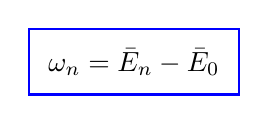
\begin{tikzpicture}
  \node[draw=blue,line width=0.9pt,inner sep=7pt]
    {$\omega_n=\bar E_n-\bar E_0$};
\end{tikzpicture}
\end{center}

\YinLine{$e.g.$ from}
\[
 \widetilde G(k)=\frac{1}{k^2+1+\frac{g}{4}
 -\frac{g^2}{8}\left(\frac{1}{4}+\frac{1}{k^2+9}\right)
 +\ldotp\ldotp\ldotp\ldotp,}
\]
\YinLine{we expect the first pole to be near $k\simeq i$,}
\[
 \omega_1=1+\frac{g}{8}-\frac{g^2}{32}+O(g^3).
\]
\begin{center}
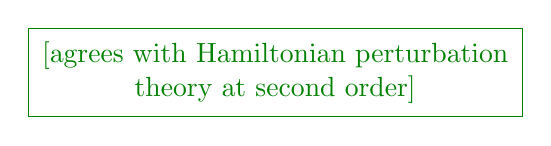
\begin{tikzpicture}
  \node[blue] at (0,0) {$\checkmark$};
  \node[green!50!black,draw=green!50!black,inner sep=5pt,align=center]
    at (2.2,0) {[agrees with Hamiltonian perturbation\\ theory at second order]};
\end{tikzpicture}
\end{center}

\begin{center}
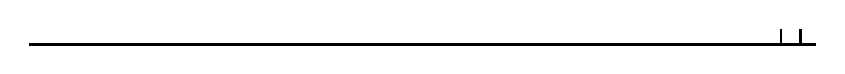
\begin{tikzpicture}
  \draw[line width=0.8pt] (-5,0)--(5,0);
  \draw[line width=0.8pt] (4.55,0)--(4.55,0.2);
  \draw[line width=0.8pt] (4.8,0)--(4.8,0.2);
\end{tikzpicture}
\end{center}

\begin{center}
  \underline{Example 3:}
\end{center}
\[
 L=\frac{1}{2}\dot q^{\,2}-\frac{1}{2}q^2-\frac{g}{8}q^2\dot q^{\,2}
\]
\[
 p=\frac{\partial L}{\partial\dot q}
 =\dot q\left(1-\frac{g}{4}q^2\right)
\]
\[
 H=\dot q\,p-L
\]
\[
 =\frac{1}{2}\left(1-\frac{g}{4}q^2\right)^{-1}p^2+\frac{1}{2}q^2.
\]

% AMBIGUITY P54-A1: the repeated dots and comma after the example denominator,
% the two right-hand divider marks, and the exact Res placement remain open.
% See work/253a-ch02/ambiguities.md.
% PAGE-TRANSITION: physical p. 54 leaves Example 3 open after H; physical
% p. 55 changes variables and asks ``ordering in quantization ?''.

% ---------------------------------------------------------------------------
\YinPageBoundary{44}{55}

\begin{center}
\begin{tikzpicture}[>=Stealth]
  \draw[magenta,->,line width=0.9pt] (0,0)--(0.3,0.55);
  \node[magenta] at (1.5,0.45) {ordering in quantization ?};
\end{tikzpicture}
\end{center}

\YinGray{\YinLine{$*$ Can also consider a change of variable}}
\[
 \dot y=\sqrt{1-\frac{g}{4}\phi^2}\,\dot\phi
\]
\[
 y=\phi-\frac{g}{24}\phi^3+\cdots
\]
\YinGray{\YinLine{and rewrite $L\longrightarrow L(y,\dot y)$}}
\[
 =\frac{\dot y^{\,2}}{2}-V(y),
\]
\[
 V(y)=\frac{1}{2}y^2+\frac{g}{24}y^4+\cdots
\]
\YinGray{\YinLine{Same as anharmonic oscillator up}}
\YinGray{\YinLine{to $O(g^2)$ corrections to the potential.}}

\YinGray{\YinLine{But, we will insist on working with the}}
\YinGray{\YinLine{$\phi$-variable in the path integral, and}}
\YinGray{\YinLine{see what happens ...}}

% AMBIGUITY P55-A1: the magenta question and its upward arrow have no
% recoverable referent. The phi/varphi glyph is retained as phi. See
% work/253a-ch02/ambiguities.md.
% PAGE-TRANSITION: physical p. 55 turns from the change of variable back to
% the phi-variable in the path integral; physical p. 56 begins its Euclidean
% Lagrangian and integration-by-parts decomposition.

% ---------------------------------------------------------------------------
\YinPageBoundary{45}{56}

\[
 L^E=\frac{1}{2}(\partial_\tau\phi)^2+\frac{1}{2}\phi^2
 -\frac{1}{8}g\phi^2(\partial_\tau\phi)^2
\]
\begin{center}

\begin{tikzpicture}
  \draw[purple,line width=0.9pt,decorate,
    decoration={brace,amplitude=4pt,mirror}] (-1.0,0)--(2.8,0);
  \node[purple] at (0.9,-0.45) {\textquotedblleft\ \textquotedblright};
\end{tikzpicture}
\end{center}

\YinPurple{\[
 -\frac{g}{24}\partial_\tau(\phi^3\partial_\tau\phi)
 +\frac{g}{24}\phi^3\partial_\tau^2\phi
\]}
\begin{center}

\begin{tikzpicture}
  \draw[magenta,line width=0.8pt,decorate,
    decoration={brace,amplitude=3pt,mirror}] (-2.7,0)--(-0.1,0);
  \node[magenta] at (-1.4,-0.45) {total derivative};
  \node[magenta] at (-0.9,-0.9) {does not contribute to $S^E$};
  \draw[red,line width=0.8pt,decorate,
    decoration={brace,amplitude=3pt,mirror}] (0.3,0)--(2.7,0);
  \node[red] at (1.5,-0.45) {can keep just this};
\end{tikzpicture}
\end{center}

\YinLine{up to first order in $g$,}
\[
 \langle\phi(\tau)\,\phi(0)\rangle
\]
\begin{center}
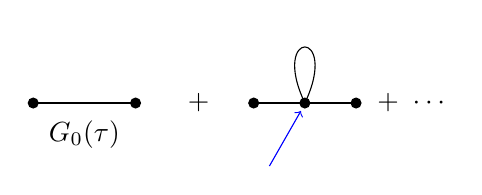
\begin{tikzpicture}[x=1cm,y=1cm]
  \fill (0,0) circle (2pt); \fill (1.3,0) circle (2pt);
  \draw (0,0)--(1.3,0); \node at (0.65,-0.4) {$G_0(\tau)$};
  \node at (2.1,0) {$+$};
  \fill (2.8,0) circle (2pt); \fill (4.1,0) circle (2pt);
  \draw (2.8,0)--(4.1,0); \fill (3.45,0) circle (2pt);
  \draw (3.45,0) .. controls (3.0,0.95) and (3.9,0.95) .. (3.45,0);
  \draw[blue,->] (3.0,-0.8)--(3.4,-0.1);
  \node at (4.8,0) {$+\ \cdots$};
\end{tikzpicture}
\end{center}

\YinBlue{\[
 \phi(\tau)\,\phi(0)\cdot\frac{g}{8}
 \int d\tau'\,(\phi(\tau'))^2(\partial_{\tau'}\phi(\tau'))^2
\]}
\begin{center}

\begin{tikzpicture}
  \draw[magenta,line width=0.8pt,decorate,
    decoration={brace,amplitude=3pt,mirror}] (-3.4,0)--(2.8,0);
  \draw[magenta,line width=0.8pt,decorate,
    decoration={brace,amplitude=3pt,mirror}] (-1.0,0.18)--(1.5,0.18);
  \draw[magenta,line width=0.8pt,decorate,
    decoration={brace,amplitude=3pt,mirror}] (2.0,0.18)--(3.4,0.18);
\end{tikzpicture}
\end{center}
\YinMagenta{\YinLine{+ various other contractions}}
\YinLine{Can represent as several diagrams}
\begin{center}
\begin{tikzpicture}[>=Stealth]
  \draw[->,line width=0.8pt] (0,0)--(1.0,0.85);
\end{tikzpicture}
\end{center}

% Six lower one-vertex line-and-loop drawings. The blue marks are derivative
% insertions; the first drawing retains the tau, tau', 0 labels and arrow.
\begin{center}
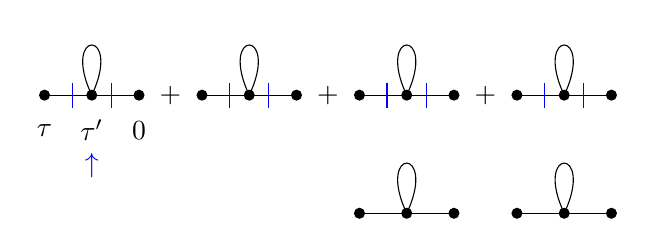
\begin{tikzpicture}[x=1cm,y=1cm]
  \foreach \x/\y in {0/0,2.0/0,4.0/0,4.0/-1.5,6.0/0,6.0/-1.5} {
    \fill (\x,\y) circle (2pt); \fill (\x+1.2,\y) circle (2pt);
    \draw (\x,\y)--(\x+1.2,\y); \fill (\x+0.6,\y) circle (2pt);
    \draw (\x+0.6,\y) .. controls (\x+0.2,\y+0.85)
      and (\x+1.0,\y+0.85) .. (\x+0.6,\y);
  }
  \draw[blue] (0.35,0.16)--(0.35,-0.16); \draw[blue] (0.85,0.16)--(0.85,-0.16);
  \draw[blue] (2.35,0.16)--(2.35,-0.16); \draw[blue] (2.85,0.16)--(2.85,-0.16);
  \draw[blue] (4.35,0.16)--(4.35,-0.16); \draw[blue] (4.85,0.16)--(4.85,-0.16);
  \draw[blue] (6.35,0.16)--(6.35,-0.16); \draw[blue] (6.85,0.16)--(6.85,-0.16);
  \node at (0,-0.45) {$\tau$}; \node at (0.6,-0.45) {$\tau'$};
  \node at (1.2,-0.45) {$0$};
  \node[blue] at (0.6,-0.9) {$\uparrow$};
  \node at (1.6,0) {$+$}; \node at (3.6,0) {$+$};
  \node at (5.6,0) {$+$};
\end{tikzpicture}
\end{center}

% AMBIGUITY P56-A1: the purple brace-like mark under the interaction and the
% exact derivative-leg assignment in the six diagrams are visual readings.
% See work/253a-ch02/ambiguities.md.
% PAGE-TRANSITION: physical p. 56 ends with the first-order contraction row;
% physical p. 57 begins with the explicit 2-times contraction.

% ---------------------------------------------------------------------------
\YinPageBoundary{46}{57}

% A disconnected tall blue curved continuation stroke sits at the upper left.
\begin{center}

\begin{tikzpicture}
  \draw[blue,line width=1.0pt] (0,0.8) .. controls (-0.35,0.4)
    and (-0.35,-0.1) .. (0,-0.45);
\end{tikzpicture}
\end{center}

\YinPurple{$2\times$}\quad
\YinBlue{$g(\tau)g(0)\cdot\frac{g}{8}\int d\tau'
 g(\tau-\tau')g(\tau')\partial g(\tau')\partial g(\tau')$}

\begin{center}

\begin{tikzpicture}
  \draw[magenta,line width=0.8pt,decorate,
    decoration={brace,amplitude=3pt}] (-3.7,0)--(0.2,0);
  \draw[magenta,line width=0.8pt,decorate,
    decoration={brace,amplitude=3pt}] (-2.6,0.18)--(-0.8,0.18);
  \draw[magenta,line width=0.8pt,decorate,
    decoration={brace,amplitude=3pt}] (-0.2,0.18)--(0.55,0.18);
  \draw[magenta,line width=0.8pt,decorate,
    decoration={brace,amplitude=3pt}] (0.4,0.18)--(2.0,0.18);
\end{tikzpicture}
\end{center}

\[
 =\frac{g}{4}\int d\tau'\,G_0(\tau-\tau')G_0(\tau')
 \left(-\partial^2G_0(0)\right)
\]
\[
 =\frac{g}{4}\int\frac{dk}{2\pi}\frac{e^{ik\tau}}{(k^2+1)^2}
 \int\frac{dk'}{2\pi}\frac{k'^2}{k'^2+1}.
\]
\begin{center}
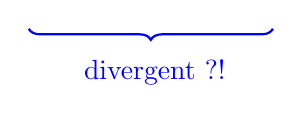
\begin{tikzpicture}
  \draw[blue,line width=0.8pt,decorate,
    decoration={brace,amplitude=4pt,mirror}] (-0.8,0)--(2.3,0);
  \node[blue] at (0.8,-0.55) {divergent ?!};
\end{tikzpicture}
\end{center}
\YinIndigo{\[
 G_0(\tau)=\frac{1}{2}e^{-|\tau|}
\]}
\YinIndigo{\[
 -\partial^2G_0(0)=\infty
\]}
\YinRed{\YinLine{?!}}

\YinGray{\YinLine{The other contributions are finite:}}
\begin{center}
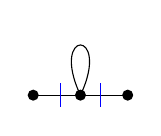
\begin{tikzpicture}[x=1cm,y=1cm]
  \fill (0,0) circle (2pt); \fill (1.2,0) circle (2pt);
  \draw (0,0)--(1.2,0); \fill (0.6,0) circle (2pt);
  \draw (0.6,0) .. controls (0.2,0.85) and (1.0,0.85) .. (0.6,0);
  \draw[blue] (0.35,0.15)--(0.35,-0.15); \draw[blue] (0.85,0.15)--(0.85,-0.15);
\end{tikzpicture}
\YinGray{$\displaystyle =\frac{g}{4}\int\frac{dk}{2\pi}
 \frac{e^{ik\tau}}{(k^2+1)^2}\cdot k^2
 \int\frac{dk'}{2\pi}\frac{1}{k'^2+1}.$}
\end{center}

\begin{center}
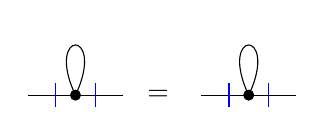
\begin{tikzpicture}
  \draw (0,0)--(1.2,0); \fill (0.6,0) circle (2pt);
  \draw (0.6,0) .. controls (0.2,0.85) and (1.0,0.85) .. (0.6,0);
  \draw[blue] (0.35,0.15)--(0.35,-0.15); \draw[blue] (0.85,0.15)--(0.85,-0.15);
  \node at (1.65,0) {$=$};
  \draw (2.2,0)--(3.4,0); \fill (2.8,0) circle (2pt);
  \draw (2.8,0) .. controls (2.4,0.85) and (3.2,0.85) .. (2.8,0);
  \draw[blue] (2.55,0.15)--(2.55,-0.15); \draw[blue] (3.05,0.15)--(3.05,-0.15);
\end{tikzpicture}
\end{center}
\YinGray{\[
 =\frac{g}{2}\int\frac{dk}{2\pi}\frac{e^{ik\tau}}{(k^2+1)^2}\cdot ik
 \int\frac{dk'}{2\pi}\frac{ik'}{k'^2+1}=0
\]}
\begin{center}
\YinGray{by symmetry}
\end{center}

\YinGray{\YinLine{Same for}}
\begin{center}
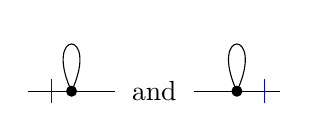
\begin{tikzpicture}
  \draw (0,0)--(1.1,0); \fill (0.55,0) circle (2pt);
  \draw (0.55,0) .. controls (0.18,0.8) and (0.92,0.8) .. (0.55,0);
  \draw[blue] (0.3,0.15)--(0.3,-0.15);
  \node at (1.6,0) {and};
  \draw (2.1,0)--(3.2,0); \fill (2.65,0) circle (2pt);
  \draw (2.65,0) .. controls (2.28,0.8) and (3.02,0.8) .. (2.65,0);
  \draw[blue] (3.0,0.15)--(3.0,-0.15);
\end{tikzpicture}
\end{center}

% AMBIGUITY P57-A1: the top derivative line retains unsubscripted partials;
% the isolated blue stroke and the unlabelled contraction groupings remain
% visual source marks. See work/253a-ch02/ambiguities.md.
% PAGE-TRANSITION: physical p. 57 moves from the divergent coincident term
% to the finite contractions; physical p. 58 explains the measure cutoff.

% ---------------------------------------------------------------------------
\YinPageBoundary{47}{58}

\YinLine{The divergence is due to $\int$ at large $k$.}
\YinLine{The origin of this divergence lies in}
\YinLine{the path integral measure}
\[
 [Dg]=\prod_k d\widetilde g_k
\]
\YinGray{\[
 g(\tau)=\int\frac{dk}{2\pi}\,\widetilde g(k)e^{ik\tau}
\]}

\begin{center}
\begin{tikzpicture}[>=Stealth]
  \node at (0,0) {$[Dg]$};
  \draw[red,->,line width=0.9pt] (0,-0.4)--(0,-1.0);
  \node[red] at (0.9,-0.7) {regularization};
  \node at (0,-1.5) {$\displaystyle\prod_{|k|<\YinRed{\Lambda}}d\widetilde g_k$};
\end{tikzpicture}
\end{center}

\begin{center}
\begin{tikzpicture}[>=Stealth]
  \fill (0,0) circle (2pt); \fill (3.0,0) circle (2pt);
  \draw (0,0)--(3.0,0); \fill (1.5,0) circle (2pt);
  \draw (1.5,0) .. controls (1.0,1.0) and (2.0,1.0) .. (1.5,0);
  \draw[blue,->] (0.9,-0.25)--(0.35,-0.25);
  \draw[blue,->] (2.2,-0.25)--(1.7,-0.25);
  \draw[blue,->] (1.2,0.8)--(1.0,0.35);
  \node[blue] at (0.6,-0.6) {$k$}; \node[blue] at (2.1,-0.6) {$k$};
  \node[blue] at (1.1,1.15) {$k'$};
\end{tikzpicture}
\end{center}
\YinLine{Effectively cuts off the $k'$}
\YinLine{\textquotedblleft loop\textquotedblright integral by $|k'|<\YinRed{\Lambda}$,}
\begin{center}
\YinMagenta{$[\text{will eventually take }\Lambda\to\infty\ \ldotp\ldotp\ldotp]$}
\end{center}

\[
 \langle g(\tau)g(0)\rangle\equiv G(\tau)
 =\int\frac{dk}{2\pi}\frac{e^{ik\tau}}{k^2+1-\Sigma(k)}
\]

% AMBIGUITY P58-A1: retain the bare integral in the opening sentence, the
% distinction between d\widetilde g_k and \widetilde g(k), and the three-dot
% future-limit note. See work/253a-ch02/ambiguities.md.
% PAGE-TRANSITION: physical p. 58 ends with the dressed propagator; physical
% p. 59 begins ``With the cutoff regularization,'' and evaluates Sigma(k).

% ---------------------------------------------------------------------------
\YinPageBoundary{48}{59}

\YinLine{With the cutoff regularization,}
\[
\begin{aligned}
 \Sigma(k)={}&\frac{g}{4}\int_{|k'|<\YinRed{\Lambda}}
 \frac{dk'}{2\pi}\frac{k'^2}{k'^2+1}
 +\frac{g}{4}k^2\int\frac{dk'}{2\pi}\frac{1}{k'^2+1}
 +O(g^2)
\end{aligned}
\]
\begin{center}
\begin{tikzpicture}
  \draw[blue,line width=0.8pt,decorate,
    decoration={brace,amplitude=3pt,mirror}] (-0.2,0)--(2.0,0);
  \node[blue] at (0.9,0.45) {$\frac{1}{2}$};
\end{tikzpicture}
\end{center}
\[
 =\frac{g}{4}\left(\frac{k^2}{2}+\frac{\YinRed{\Lambda}}{\pi}
 -\frac{1}{2}+O(\Lambda^{-1})\right)+O(g^2)
\]

\YinLine{$*$ What is the interpretation of $\Lambda\to\infty$ ?}
\YinLine{$-$ Nothing wrong with QM w/}
\[
 H=\frac{1}{2}\left(1-\frac{g}{4}q^2\right)^{-1}p^2+\frac{1}{2}q^2
\]
\YinGray{\YinLine{(at least for $g<0$)}}
\YinLine{except for potential ordering ambiguity}
\YinLine{....}

\YinLine{To understand what's going on,}
\YinLine{let us restore $\hbar$-dependence;}
\[
 Z=\int[Dq]\exp\left[-\frac{1}{\YinBlue{\hbar}}
 \int d\tau\,L^E\right]
\]

% AMBIGUITY P59-A1: the second self-energy integral has no visible cutoff
% subscript; the blue 1/2 is an annotation over that integral. Preserve both.
% AMBIGUITY P59-A2: retain the four dot-like marks after ordering ambiguity.
% See work/253a-ch02/ambiguities.md.
% PAGE-TRANSITION: physical p. 59 restores hbar-dependence and hands off to
% physical p. 60, which questions an O(hbar) correction and introduces
% counter terms.

% ---------------------------------------------------------------------------
\YinPageBoundary{49}{60}

\[
 L^E=\frac{(\partial_\tau q)^2}{2}+\frac{q^2}{2}
 -\frac{1}{8}gq^2(\partial_\tau q)^2+\YinBlue{O(\hbar)\ ?}
\]
\begin{center}
\begin{tikzpicture}[>=Stealth]
  \draw[blue,->] (1.1,0.7)--(1.1,0.1);
  \node[blue,align=left] at (2.5,0.9)
    {possible corrections\\ needed for agreement\\ with quantum Hamiltonian?};
\end{tikzpicture}
\end{center}
\YinMagenta{\YinLine{\textquotedblleft Counter terms\textquotedblright}}

\[
 \widetilde G(k)=\frac{\YinGray{\hbar}}{k^2+1-\Sigma(k)}\ ,
\]
\[
 \Sigma(k)=\frac{\YinGray{\hbar}g}{4}
 \left(\frac{k^2}{2}+\frac{\YinRed{\Lambda}}{\pi}-\frac{1}{2}
 +O(\Lambda^{-1})\right)+O(\YinGray{\hbar^2g^2})
\]

\YinLine{Indeed, if we include}
\[
 \Delta L^E=\YinMagenta{c}\cdot g\YinGray{\hbar}\frac{q^2}{2}\ ,
\]

\begin{center}
\begin{tikzpicture}[>=Stealth]
  \node at (-1.4,0) {$\Sigma(k)=$};
  \draw[gray] (-0.2,0)--(0.5,0);
  \draw[black,line width=1.0pt] (0.5,0) ellipse (0.7 and 0.42);
  \node at (0.5,0) {1PI};
  \draw[gray] (1.2,0)--(1.9,0);
  \draw[blue,->] (-0.15,0.55)--(0.2,0.15);
  \draw[blue,->] (1.85,0.55)--(1.5,0.15);
  \node[blue] at (0.0,0.7) {$k$}; \node[blue] at (1.7,0.7) {$k$};
\end{tikzpicture}
\end{center}
\YinLine{$\Sigma(k)$ receives an extra contribution
  $-\YinMagenta{c}\cdot g\YinGray{\hbar}$}
\YinLine{at order $g$, giving the result}
\[
 \Sigma(k)=\YinGray{\hbar}g\left(\frac{k^2}{8}
 +\frac{\YinRed{\Lambda}}{4\pi}-\frac{1}{8}-\YinMagenta{c}
 +O(\Lambda^{-1})\right)
\]
\[
 +O(g^2)
\]

% AMBIGUITY P60-A1: preserve the questioned +O(hbar) term and the visible
% mismatch between O(hbar^2 g^2) and the final O(g^2). See
% work/253a-ch02/ambiguities.md.
% PAGE-TRANSITION: physical p. 60 ends after the counterterm-improved Sigma;
% physical p. 61 chooses c and identifies the finite-part ambiguity.

% ---------------------------------------------------------------------------
\YinPageBoundary{50}{61}

\YinLine{$*$ The path integral is only \YinRed{defined} provided}
\YinLine{regularization via the cutoff \YinRed{$\Lambda$}.}

\YinLine{Choosing $\YinMagenta{c}=\frac{\YinRed{\Lambda}}{4\pi}+\text{finite},$ and}
\YinLine{take the limit $\YinRed{\Lambda}\to\infty$ in the end,}
\YinLine{we find a finite result for $\Sigma(k)$.}

\YinLine{$*$ The finite part of $\YinMagenta{c}$ represents an}
\YinLine{ambiguity in quantization, i.e. the}
\YinLine{possibility of adjusting the quantum}
\YinLine{Hamiltonian by a term of order $\hbar$.}

\[
 \widetilde G(k)=\frac{\YinGray{\hbar}}{k^2+1-\Sigma(k)}
 \quad\text{has pole at } k=i\omega_1,
\]
\[
 \omega_1=1+\YinGray{\hbar}g\left(-\frac{\Lambda}{8\pi}
 +\frac{c}{2}+\frac{1}{8}\right)+O(g^2).
\]
\[
 =\widehat E_1-\widehat E_0
\]

% AMBIGUITY P61-A1: retain the source colors on defined, c, Lambda, and
% hbar, and retain hats on both E symbols in the final energy relation. See
% work/253a-ch02/ambiguities.md.
% PAGE-TRANSITION: physical p. 61 ends with omega_1=Ehat_1-Ehat_0;
% physical p. 62 begins the hyphenated continuation ``- energy gap''.

% ---------------------------------------------------------------------------
\YinPageBoundary{51}{62}

\YinLine{$-$ energy gap, unambiguous physical}
\YinLine{observable regardless of the interpretation}
\YinLine{of $g(c)$.}

\YinLine{$*$ The Counter terms, together with}
\YinLine{regularization scheme, should be viewed as}
\YinLine{part of the definition of the path integral.}

\begin{center}
\begin{tikzpicture}
  \draw[line width=0.8pt] (-4.5,0)--(3.9,0);
  \draw[line width=0.8pt] (4.15,0)--(4.15,0.18);
  \draw[line width=0.8pt] (4.38,0)--(4.38,0.18);
\end{tikzpicture}
\end{center}

\YinLine{To fix the finite part of the Counter}
\YinLine{terms require additional physical input,}
\YinLine{$e.g.$ symmetries of the quantum Hamiltonian}
\YinLine{In general QM, anything goes in $H$}
\YinLine{In QFT, Poincar\'e sym $+$ Causality}
\YinLine{highly restrictive !}

% AMBIGUITY P62-A1: the two short marks after the horizontal rule are
% retained as unresolved visual punctuation. Preserve the source grammar,
% capitalization, and the space before the exclamation point. See
% work/253a-ch02/ambiguities.md.
% PAGE-TRANSITION: physical p. 62 is the terminal note page for Chapter 2;
% assignment material begins on physical p. 63.
